\section{Energy Plane electronics}\label{sec:energy_fee}
After the firsts test with the PMTs and the whole electronic chain at LSC, two important issues were identified in the first design of the electronic chain: 
\begin{itemize}
\item The impedance of the high voltage differential cable was not well matched with the entering impedance of the de-coupling board of the FEE.
\item The decoupling capacitor was producing a negative overshoot in the signal that resulted in undesirable bipolar signals. 
\end{itemize}

These problems were not present in NEXT-DEMO since:
\begin{itemize}
\item Cable length was in the order of 1 m, so transmission line effects were not evident, unlike in the 10 m cable used for NEW.
\item Decoupling capacitors were not required, as a grounded-anode configuration was used. In NEW, a grounded-cathode scheme was chosen, so that the PMT bodies could at ground, in order to avoid problems with electrical insulation. 
\end{itemize}

To solve the above two issues, a full re-design of the bases and the FEE of the energy plane has taken place over the last two months. 
The new base design includes some of the components that were in the decoupling board previously. Other changes in the base are:

\begin{itemize}
\item The resistor chain has been slightly modified following the manufacturer (Hamamatsu) recommendations. 
\item Series resistors in the anode and in the last dynode have been added with the aim to damp reflections in the signal.
\item Capacitance values between dynodes have been modified to reduce the gain compression in the PMT for large signals.
\end{itemize}

Figure \ref{fig:fee_scheme} shows the new design for the front-end circuit. The main modifications to the previous design are:

\begin{itemize}
\item Differential and common-mode mode terminations have been added to the first stage's input. This has forced to change the first stage's topology.
\item In order to recover the signal's DC level and thus avoid bipolar pulses, an active integrator has been implemented in the second stage of the FEE.
\end{itemize}

The current circuit mitigates most of the problems but adds a new one: the integrator introduces a low-frequency (up to 10 kHz) walk in the signal's baseline.

The effect on the low-amplitude narrow S1 signal used for trigger can be minimized with a moving-average filter in the FPGA in the DAQ modules, 
which dynamically computes the baseline for each channel and subtracts it from the signal. At the time of writing this report, tests with actual PMT signals produce good results.

The effect on the larger-amplitude, wide (up to 100 microseconds) S2 signal used to measure energy is potentially more severe, as the baseline correction cannot be performed.
Aceptable signal-to-noise ratios (S/N) are expected with a number of enhancements which are currently being implemented. 
As an example, a factor of three in the S/N will be achieved just by replacing the current de-coupling capacitors with larger 8 nF ones. 

In the first half of May 2016, the new front-end circuit will be installed and tested in the NEW detector readout.

\begin{figure}
  \begin{center}
    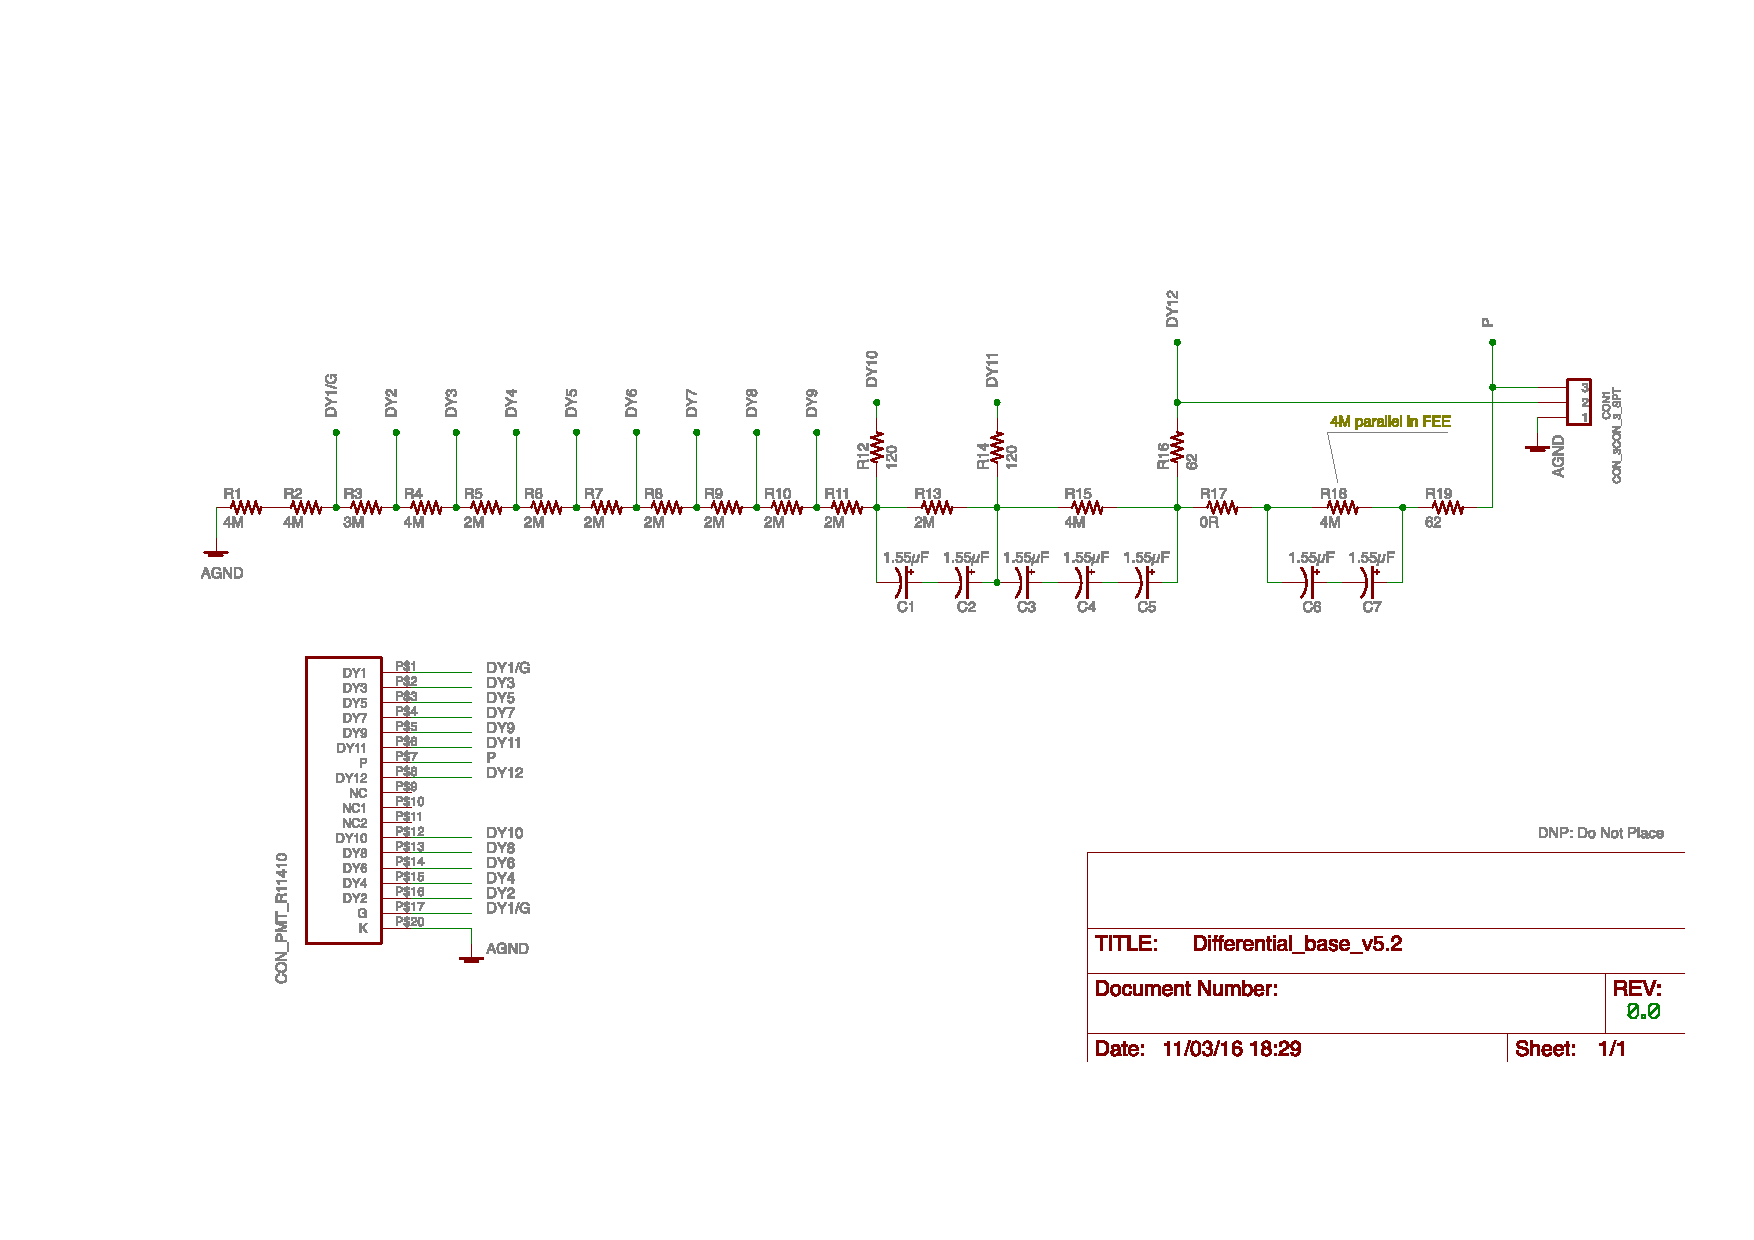
\includegraphics[height=4cm,width=0.95\textwidth]{img/Differential_base}
    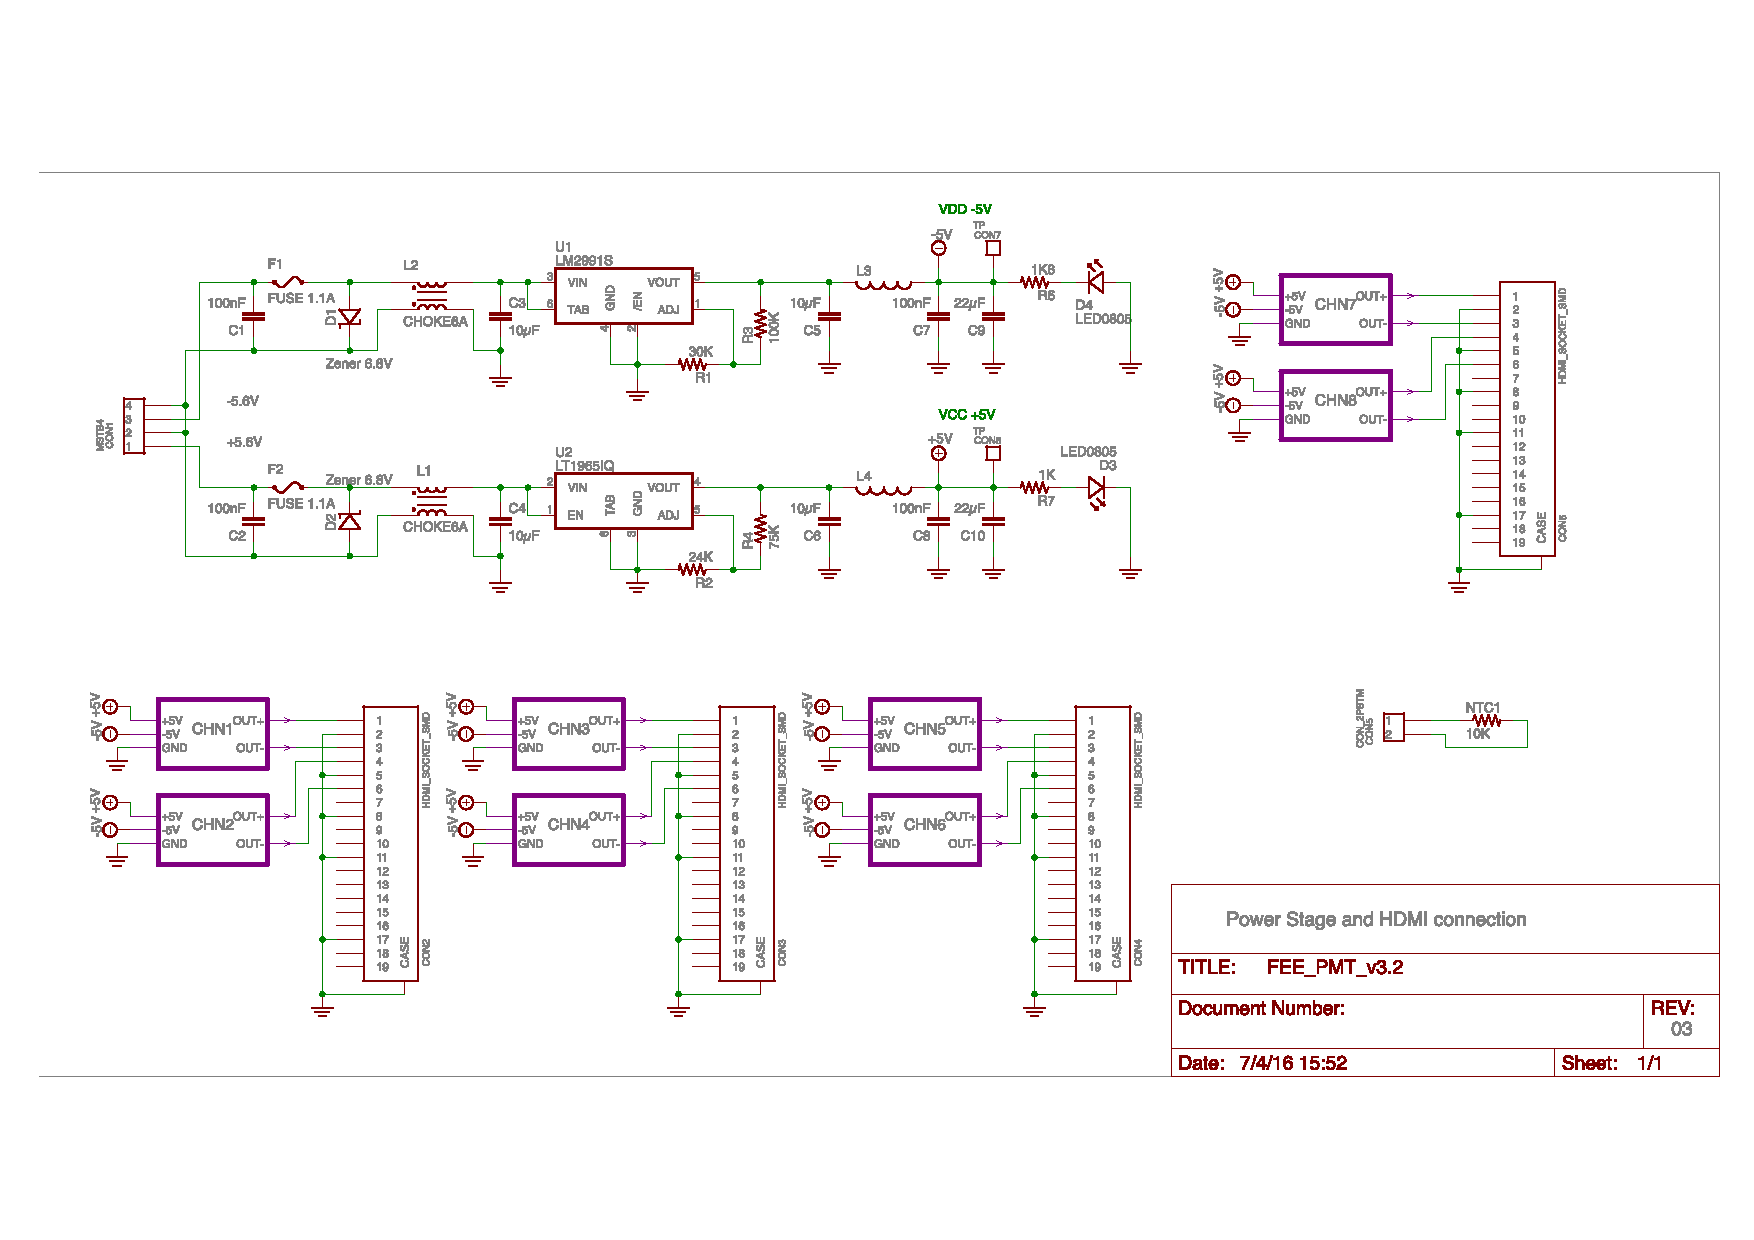
\includegraphics[height=4cm,width=0.95\textwidth]{img/de-coupling_board}
	  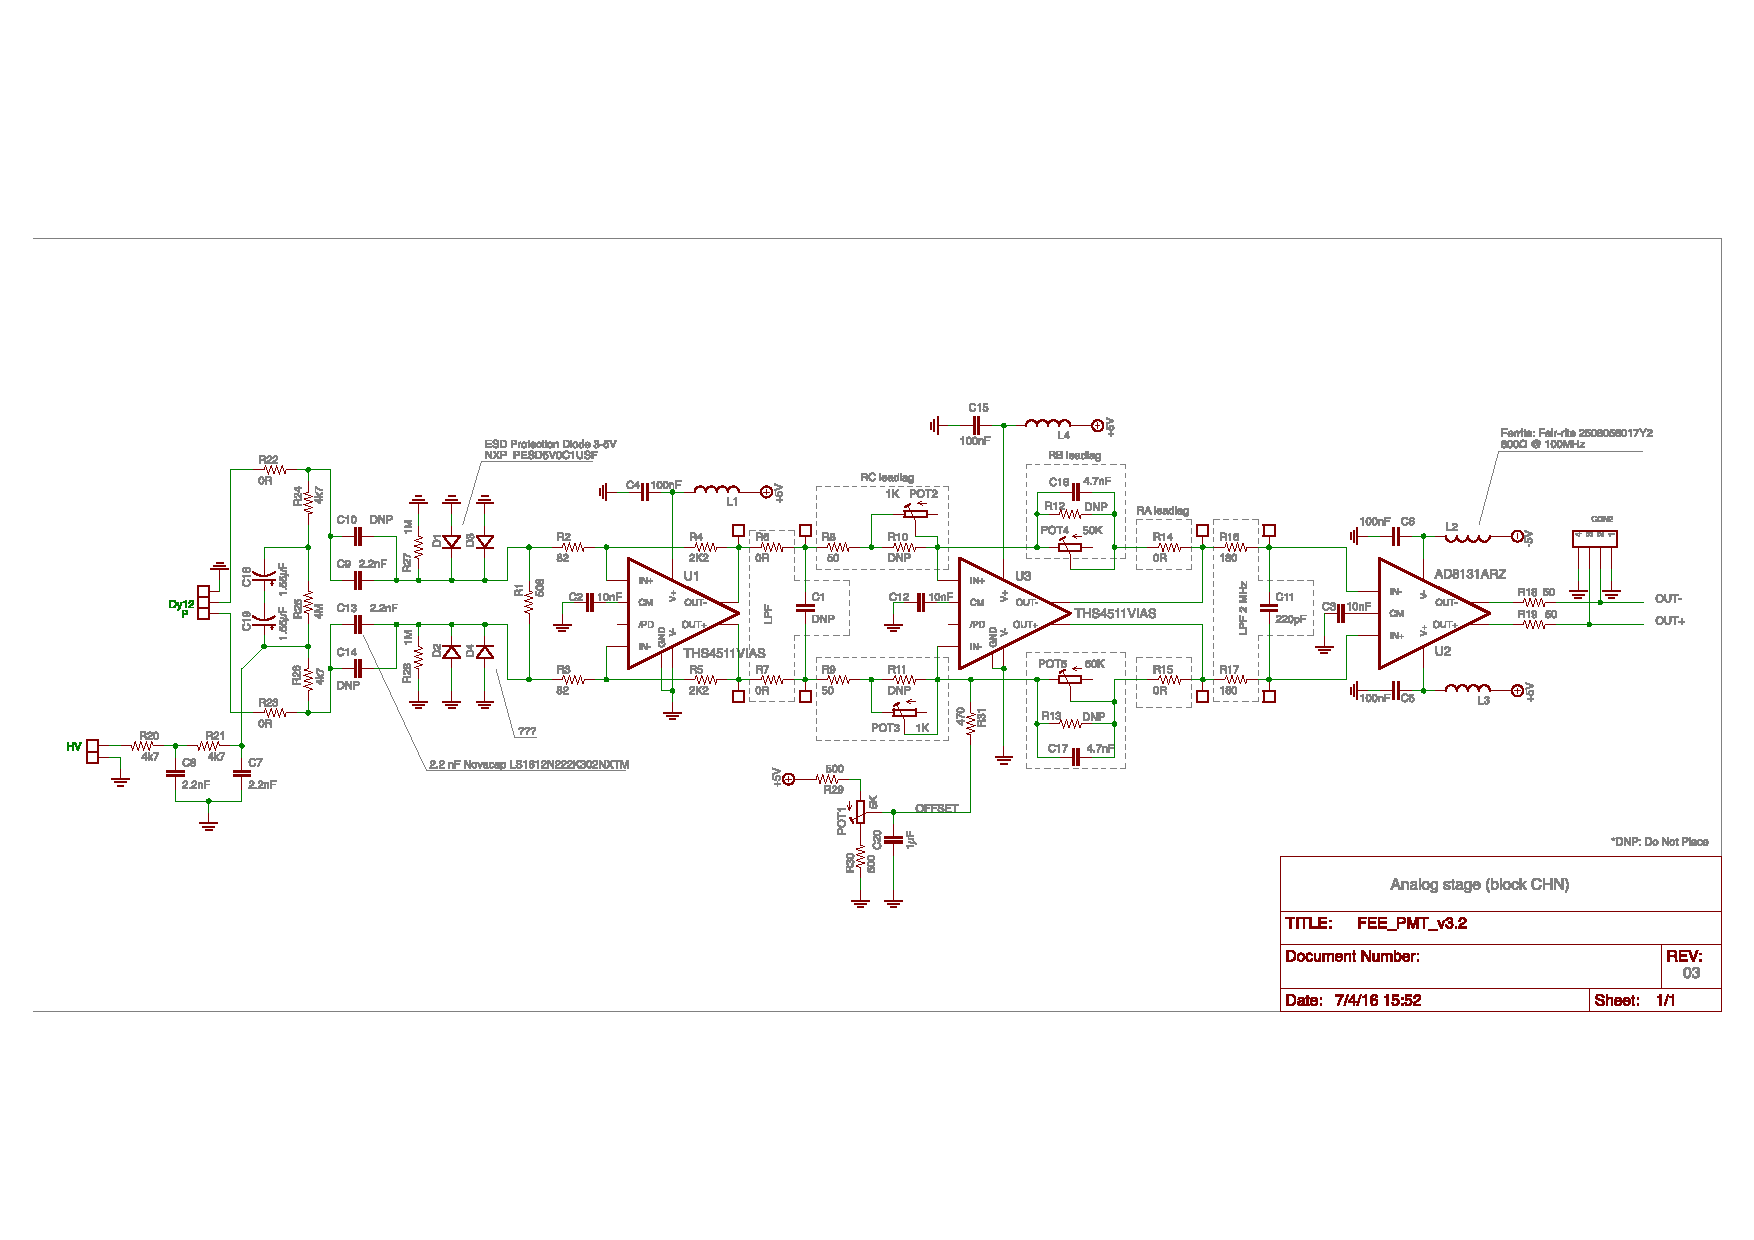
\includegraphics[height=4cm,width=0.95\textwidth]{img/FEE_PMT}
  \end{center}
  \caption{Schematics of the energy plane electronics. From top to bottom: Differential base (top), voltage regulators and four 2-channel hyerarchical blocks (middle) and one front-end channel circuit topology (bottom).  }
  \label{fig:fee_scheme} 
\end{figure}

There is more room for improvement by moving the first stage in the amplifier to the PMT base, as in this case larger resistors can be used and noise will be much lower. 
This is possible because there is no need to match impedances, as the amplifier would be very close to the base. The described approach will be explored in Spring 2016, in parallel to the tests
of the new front-end shown in figure \ref{fig:fee_scheme}.

\begin{figure}
  \begin{center}
    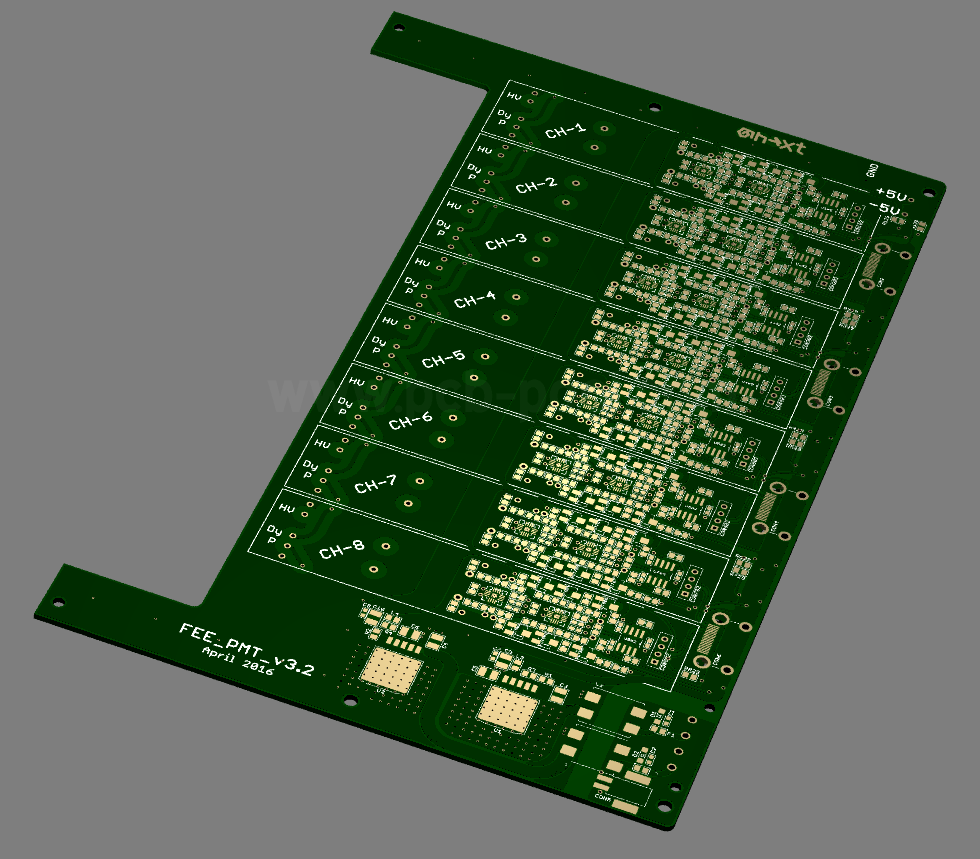
\includegraphics[height=8cm,width=0.95\textwidth]{img/FEE_PMT_PCB}
  \end{center}
  \caption{New PMT front-end PCB board, currently under production}
  \label{fig:fee_pcb_scheme} 
\end{figure}